\documentclass[a4paper,12pt]{article}
\usepackage{graphicx}
%\usepackage{natbib}

\usepackage[utf8]{inputenc}
\usepackage[T1]{fontenc}
%\usepackage[french]{babel}

\usepackage[colorlinks,bookmarks=false,linkcolor=blue,urlcolor=blue,citecolor=black]{hyperref}
\usepackage{amsmath}
\usepackage{amssymb}
\usepackage{mathrsfs}
\usepackage{textcomp}

\graphicspath{{./images/}}

\usepackage{hhline}
\usepackage{caption}
\usepackage{float}

\newcommand{\mail}[1]{{\href{mailto:#1}{#1}}}
\newcommand{\ftplink}[1]{{\href{ftp://#1}{#1}}}

\newcommand{\derivt}[1]{\frac{\partial}{\partial t} #1}
\newcommand{\derivr}[1]{\frac{\partial}{\partial r} #1}

\usepackage[scale=0.75]{geometry}
%\usepackage[top=2.48cm, bottom=1.5cm, left=2cm, right=2cm]{geometry}

\usepackage{listings}
\usepackage{subfig}

\usepackage{listings}
\usepackage{color}

\usepackage{enumerate}
\usepackage{hyperref}
 
\definecolor{codegreen}{rgb}{0,0.6,0}
\definecolor{codegray}{rgb}{0.5,0.5,0.5}
\definecolor{codepurple}{rgb}{0.58,0,0.82}
\definecolor{backcolour}{rgb}{0.95,0.95,0.92}
 
\lstdefinestyle{mystyle}{
    backgroundcolor=\color{backcolour},   
    commentstyle=\color{codegreen},
    keywordstyle=\color{magenta},
    numberstyle=\tiny\color{codegray},
    stringstyle=\color{codepurple},
    basicstyle=\footnotesize,
    breakatwhitespace=false,         
    breaklines=true,                 
    captionpos=b,                    
    keepspaces=true,                 
    numbers=left,                    
    numbersep=5pt,                  
    showspaces=false,                
    showstringspaces=false,
    showtabs=false,                  
    tabsize=2
}



\lstset{style=mystyle}



\title{Rapport du projet de simulation numérique d'un disque d'accrétion}
\author{Mathieu de Bony, Valentin Nourry, Sylvain Cezar,\\Jérémy Couturier, Wilfried Mercier, Thomas Nicolazo}
\date{\today}



\begin{document}

\maketitle

\renewcommand{\contentsname}{Sommaire}

\newpage

\tableofcontents

\newpage

\section{Introduction}



Les trous noirs sont responsables des champs gravitationnels les plus intenses que l'on puisse trouver dans l'Univers. Lorsque ces derniers font partie d'un système binaire avec une étoile compagnon, la matière qu'ils arrachent à leur étoile s'accumule pour former des disques d'accrétions, détectables depuis la Terre grâce au rayonnement émis par la matière accélérée dans le disque. De tels systèmes sont appelé binaire X du fait que la température très élevé du disque provoquent une émission principalement dans les rayons X.

L’objectif de ce projet est de simuler numériquement en Fortran un tel disque d'accrétion pour en étudier ses caractéristiques.

\section{Description physique du modèle}

Dans notre modèle, on prend en compte divers paramètres : la masse $M$ du trou noir, $r_{\rm{min}}$ et $r_{\rm{max}}$, respectivement le plus petit rayon où les orbites sont encore stables (on précisera ce point par la suite) et le plus grand rayon caractérisant le bord extérieur du disque. Vient ensuite le taux de matière de l'étoile compagnon accrétée dans le disque $\dot M_0$, la composition chimique du disque caractérisée par les grandeurs $X$, $Y$ et $Z$ représentant respectivement la proportion d'hydrogène, d’hélium et des autres éléments plus lourd (métaux). Enfin un dernier paramètre sera $\alpha $ qui est proche de l'unité et que l'on explicitera plus loin.

On arrive donc à un total de huit paramètres, que l'on peut réduire à six. En effet, on peut exprimer $r_{\rm{min}}$ en fonction de la masse et $Z$ en fonction de $X$ et de $Y$. Cela fait donc un total de six paramètres pour décrire notre disque d'accrétion : M, $r_{\rm{max}}$, $\dot M_0$, $\alpha$, $X$ et $Y$. \\

Le seul de ces paramètres suffisant pour décrire le trou noir lui même, en supposant que l'on a un trou noir de Schwarzschild, est sa masse $M$ à partir de laquelle on définit le \textit{rayon de Schwarzschild} :
\begin{equation}
    r_s=\frac{2GM}{c^2}
\end{equation}
 avec $G$ la constante de gravitation et $c$ la vitesse de la lumière.

\subsection{Géométrie du disque}

On considère un disque à symétrie cylindrique dans l'espace repéré par les coordonnées $r$, $\phi$ et $z$. Aux vues de cette symétrie, le modèle ne portera que sur la coordonnées radiale $r$.

Comme dit plus haut, le disque s'étend de $r_{\rm{min}}$ à $r_{\rm{max}}$, tel que $r_{\rm{min}}$ soit le plus petit rayon où les orbites sont encore stables. Ce critère est donnée par la relativité générale et vaut $r_{min}=3r_s$ pour un trou noir de Schwarzschild. En dessous de cette limite, le disque est instable et la matière tombe directement vers le trou noir. Concernant $r_{\rm{max}}$, il doit d'une part être suffisamment petit pour que l'hypothèse du gaz complètement ionisé soit valide dans $[r_{\rm{min}}, r_{\rm{max}} ]$. D'autre part, il doit être assez grand pour que les ondes de matière qui se propagent radialement vers les grand $r$ s'amortissent avant d'atteindre $r_{\rm{max}}$ sous peine que les conditions au bord extérieur changeraient, ce qui rentrerait en désaccord avec le fait d'imposer des conditions aux bords.

\subsection{Phénomène d'accrétion}
Le milieu extérieur au disque, tel qu'une étoile compagnon par exemple, lui fournie une certaine quantité de matière dans un certain laps de temps. Cet apport, que l'on appelle \textit{taux d'accrétion} et qu'on note $\dot M_0$, a lieu en $r = r_{\rm{max}}$.

\subsection{Composition chimique}
Comme dit précédemment, la composition chimique est caractérisée par trois nombres sans dimensions $X$, $Y$ et $Z$, respectivement les fractions d'hydrogène, d'hélium et des métaux. Ils reliés entre eux par l'égalité $X+Y+Z=1$. Dans notre modèle, on fixera ces valeurs sur celles de la composition chimique du Soleil, à savoir :
\begin{equation}
    X=0.70,  Y=0.28, Z=0.02
\end{equation}


\subsection{Etablissement des équations}

On fait par la suite l'hypothèse que la loi de Kepler est valide. En réalité, près d'un trou noir, le champ gravitationnel est si intense qu'il faudrait l'étudier sous le point de vue de la relativité générale. Néanmoins, cette approximation képlerienne reste valide pour des orbites circulaires se situant à plus de trois rayons de Schwarzschild.\newline
Bien que la matière dans un disque d’accrétion soit censée se diriger vers le trou noir, on fait tout de même l'hypothèse que les orbites restent circulaires car la vitesse de rotation du disque est bien supérieur à la vitesse radiale $v_{\phi}$ (ou vitesse d'accrétion $v$) avec laquelle la matière tombe vers le trou noir ($v_{\phi}>>v$).

\subsubsection{La pression}

La pression du disque est causée par deux phénomènes : la pression due au gaz et celle due à la radiation.

Pour la pression de radiation, on utilise la formule
\begin{equation}
    P_{\rm{rad}}=\frac{1}{3}aT^4
\end{equation}

La pression du gaz se décompose elle-même en deux parties: la première due aux ions et la seconde due au gaz d'électrons. On supposera de plus que la température $T$ est la même pour les ions et les électrons. Pour le gaz d'ions, on a 


\begin{align*}
    P_{\rm{ion}}& =X\frac{k\rho T}{m_p} + Y\frac{k\rho T}{4m_p} + Z\frac{k\rho T}{Am_p}\\
    & =\frac{k\rho T}{m_p \mu_{\rm{ion}}}\\
    \mu_{\rm{ion}} &=\frac{1}{X+\frac{1}{4}Y+\frac{1}{A}Z}
\end{align*}



où $A$ est le nombre de masse de l'atome considéré pour un nombre de protons strictement suppérieur à 2, $m_p$ la masse du proton, $k$ est la constante de Boltzmann et $\rho$ la masse volumique.

Comme on suppose un plasma complètement ionisé, les électrons proviennent des atomes ionisés et on a un électron pour un proton et un neutron, soit, au total, $\frac{A}{2}$ électrons :

\begin{align*}
        P_{e}& =\frac{k\rho_e T}{m_e}, \quad \rho_e=m_e\big( \frac{X\rho}{m_p}\big) +2\frac{Y}{4m_p} + \frac{A}{2}\frac{Z\rho}{Am_p} \\
        & =\frac{k\rho T}{m_p \mu_{e}}, \quad \mu_e=\frac{1}{X+\frac{3}{4}Y+\frac{1}{2}Z}\\
\end{align*}

La pression du gaz totale est donc la somme de ces deux contributions, soit:


\begin{align*}
    P& = P_e+P_{ion} \xrightarrow{}\mu^{-1}=\mu_e^{-1}+\mu_{ion}^{-1}\\
    \mu^{-1} &=\big( X+\frac{1}{4}Y+\frac{1}{A}Z\big) +\big( X+\frac{1}{2}Y+\frac{1}{2}Z \big)\\
    \mu &= \frac{1}{2X+\frac{3}{4}Y+\frac{2+A}{2A}Z}
\end{align*}


$A$ est le numéro atomique des métaux, donc $A \gg 2$. Par conséquent, on peut réécrire l'équation de $\mu$ comme:

\begin{equation}
    \mu \simeq \frac{1}{2X+\frac{3}{4}Y+\frac{1}{2}Z} 
    \label{mu}
\end{equation}

Au final, pour la pression du gaz, on a : 

\begin{equation}
    P_{gaz}=\frac{\rho k T}{\mu m_p}
\end{equation}

La pression totale vaut donc :

\begin{equation}
    P=P_{gaz}+P_{rad}
\end{equation}

et on définit $\beta$ comme :

\begin{equation}
    \beta=\frac{P_{gaz}}{P}
\end{equation}

Si la pression du gaz est dominante, on aura $\beta=1$. Si, au contraire, la pression de radiation est dominante, $\beta=0$.


\subsubsection{Équation d'état}

Pour établir l'équation \eqref{mu}, on a supposé que les gaz d'ions et d'électrons sont des gaz parfaits, ce qui a permis d'écrire leur équations d'états $P_i=\frac{k\rho T}{m_i\mu_i}$. Ceci implique que le gaz reste complètement ionisé. Or, le gaz de photon est supposé être à équilibre avec la matière à la température $T$, donc cela signifie que le milieu est optiquement épais vis à vis des interactions avec les photons $(\tau_{\rm{eff}} \gg 1)$.

\subsubsection{La vitesse du son}

Le disque est donc un milieu composé de gaz et de rayonnement. On a :
\begin{equation*}
    \Gamma_1=\Big(\frac{d \ln P}{d \ln \rho}\Big)_{\rm{adiab}}=\beta + \frac{(4-3\beta)^2(\gamma_g - 1)}{12(1-\beta) )(\gamma_g -1)+\beta}
\end{equation*}

où $\gamma_g$ est l'indice adiabatique qui vaut $\gamma_g=\frac{5}{3}$ pour un gaz parfait monoatomique.

Si la pression du gaz domine $(\beta=1)$, on aura donc $\Gamma_1=\gamma_g$, et si la pression de radiation domine $(\beta=0)$, $\Gamma_1=\frac{4}{3}$.

\subsubsection{Équilibre hydrostatique}

On peut supposer que le disque est à l'équilibre hydrostatique sur l'axe $z$ si le les mouvements le long de cet axe sont subsoniques. L'équation de l'équilibre hydrostatique est $\text{\bf{grad}} P=-\rho \text{ \bf{grad}}\phi$, avec $\phi$ le potentiel gravitationnel. Puisque la masse du trou noir est très supérieur à la masse du disque, on peut écrire le potentiel comme $\phi=-\frac{GM}{D}$, avec $D=(r^2+z^2)^{\frac{1}{2}}$, $r_{\rm{min}}\le r\le r_{\rm{max}}$.
Sur l'axe des $z$ on a :
\begin{equation*}
    \frac{1}{\rho}\frac{\partial P}{\partial z}=\frac{\partial}{\partial z} \frac{GM}{(r^2+z^2)^{\frac{1}{2}}}
\end{equation*}
Sous hypothèse de disque mince, $z^2\ll r^2$, donc :

\begin{equation*}
\begin{split}
    \frac{1}{\rho}\frac{\partial P}{\partial z} &=\frac{\partial}{\partial z} \frac{GM}{r}\Big(1- \frac{z^2}{2r^2}\Big)=\frac{GM}{r}\Big( -\frac{2z}{2r^2}\Big)\\
    &=-\frac{GM}{r^3}z=-\Omega ^2z
\end{split}
\end{equation*}
où on a posé $\Omega^2 = \frac{GM}{r^3}$ la vitesse angulaire des orbites képlerienne.

On a donc :

\begin{equation*}
    \int_{P(0)}^{P(H)} dP=\int_0^H -\Omega ^2 \rho z dz
\end{equation*}

H étant la demi hauteur du disque. Si $\rho$ est constant sur $z$ de $0$ à $H$, il vient:

\begin{equation*}
    P(H)-P(0)= -\Omega ^2 \rho \frac{H^2}{2}
\end{equation*}

On définit $H$ tel que $P(H)=0$ et $P(0)$ est la pression centrale que l'on note $P_0$.
On obtient donc $P_0=\frac{1}{2}\Omega ^2\rho H^2$.

En reprenant l'équation au-dessus et en intégrant non plus de $0$ à $H$ mais de $0$ à $z$, on obtient :

\begin{equation*}
\begin{split}
    &P(z)-P(0) =-\frac{1}{2}\Omega ^2 \rho z^2\\
    \implies &P(z) =P_0-\frac{1}{2}\Omega ^2 \rho z^2=P_0\Big( 1-\frac{z^2}{H^2} \Big)
\end{split}
\end{equation*}

Prenons maintenant la valeur moyenne de la pression sur l'axe $z$:
\begin{equation*}
\begin{split}
    \langle P \rangle &= \frac{1}{H} \int_0^H P(z) dz = \frac{1}{H} \int_0^H P_0\Big( 1-\frac{z^2}{H^2}\Big) dz\\
    &=\frac{P_0}{H}\Big[ z-\frac{1}{3}\frac{z^3}{H^2} \Big]_0^H\\
    &=\frac{2}{3}P_0
\end{split}
\end{equation*}

On voit donc que $\langle P\rangle \simeq P_0$, ce qui indique que la pression dépendra surtout du rayon.

\subsubsection{Viscosité}

On considère le disque comme étant formé d'anneaux concentriques de rayon r. Le contact de ces anneaux engendre des frottements caractérisés par une certaine viscosité. Mais ces simples frottements ne suffisent pas à rendre compte de l'énergie dissipée par le disque. On fait alors appel à un autre type de viscosité, la viscosité turbulente. Cette forme de viscosité n'est pas la conséquence de frottements d'anneaux mais de tourbillons se créant dans le fluide lorsque l'écoulement devient turbulent. 

Pour la caractériser on se réfère à la théorie des disques de Shakura et Sunyaev qui nous dit que la viscosité est donnée par $\nu=\frac{2}{3}\alpha c_s H$, $\alpha $ étant un paramètre arbitraire de l'ordre de l'unité. Si cette partie est critiquable, il semble néanmoins que cette théorie soit vérifiée par des observations de binaires X. 

\subsubsection{Densité de matière}

Soient $\rho$ et $\Sigma$ respectivement la densité volumique en $[kg/m^3]$ et la densité surfacique en $[kg/m^2]$. Par définition :
\begin{equation*}
    \Sigma = 2 \int_{0}^{H}\rho (z) dz
\end{equation*}

\noindent et, aussi par définition, 
\begin{equation*}
    \langle \rho \rangle = \frac{1}{H} \int_0^H \rho (z) dz \implies \int_0^H \rho (z) dz = H \langle \rho \rangle
\end{equation*}
Donc
\begin{equation*}
     \Sigma = 2 H  \langle \rho \rangle
\end{equation*}

Si $\rho$ est constant, $ \langle \rho \rangle = \rho$. Si $\rho$ n'est pas constant, on aurait $\rho \propto  \langle \rho \rangle$ avec un facteur proche de l'unité que nous négligeons devant l'incertitude sur le paramètre $\alpha$.

\subsubsection{Évolution de la densité de matière}

On donne les équations de conservation de masse et de moment cinétique :


\begin{gather*}
    r\derivt{\Sigma} +\derivr{(\Sigma vr)} =0 \text{,\quad  pour la masse}\\
    r^2\Omega \derivt{\Sigma} + \frac{1}{r} (\Sigma r^3 \Omega v) =\frac{1}{r}\derivr{(\nu \Sigma r^3 \derivr\Omega)} \text{,\quad pour le moment cinétique}
\end{gather*}

\noindent On peut réécrire la seconde équation comme :

\begin{equation*}
    r^2\Omega \derivt {\Sigma} + r\Omega \derivr{(\Sigma vr)} + \frac{1}{r}\derivr{(r^2\Omega)} \Sigma vr=\frac{1}{r}\derivr{(\nu \Sigma r^3 \derivr\Omega)}
\end{equation*}

En se servant de la première équation, on remplace $\derivr(\Sigma vr)$ dans la seconde, ce qui donne :

\begin{equation}
\label{surface equation}
    \Sigma vr = \frac{\frac{1}{r}\derivr{(\nu \Sigma r^3 \derivr\Omega)}-r^2\Omega \derivt{\Sigma}+r^2\Omega \derivt{\Sigma}}{\frac{1}{r}\derivr{(r^2 \Omega)}}=\frac{\frac{1}{r}\derivr{(\nu \Sigma r^3 \derivr\Omega)}}{\derivr{(r^2 \Omega)}}
\end{equation}

On remplace maintenant $\Sigma vr$ dans l'équation de conservation de la masse :

\begin{gather*}
    r\derivt{\Sigma} + \derivr{\bigg \{ \frac{\derivr{(\nu \Sigma r^3 \derivr\Omega)}}{\derivr{(r^2 \Omega)}}\bigg \}}=0\\
    \Leftrightarrow \derivt{\Sigma}=-\frac{1}{r}\derivr{\bigg \{ \frac{1}{\derivr{(r^2\Omega)}} \derivr{\Big(\nu \Sigma r^3 \derivr{\Omega}\Big)} \bigg \} }
\end{gather*}

Pour des orbites képlériennes on a :

\begin{gather*}
    r^3\derivr{\Omega} = -\frac{3}{2}r^2\Omega = -\frac{3}{2}\big( GM \big)^{\frac{1}{2}}r^{\frac{1}{2}}\\
    \derivr{\big( r^2\Omega \big)} = \frac{1}{2}r\Omega = \frac{1}{2} \big( GM \big)^{\frac{1}{2}}r^{-\frac{1}{2}}
\end{gather*}

On remplace donc ces deux valeurs dans les équations précédentes et on obtient finalement :

\begin{equation*}
    \derivt{\Sigma} = \frac{3}{r}\derivr{ \big \{ r^{\frac{1}{2}} \derivr{(\nu \Sigma r^{\frac{1}{2}})} \big \}}
\end{equation*}

\subsubsection{Vitesse d'accretion}

Pour établir l'équation régissant la vitesse d'accrétion $v$, on reprend l'équation \eqref{surface equation} dans le cas képlerien :

\begin{equation*}
    \begin{split}
         \Sigma vr &= \frac{\derivr{\nu \Sigma (-\frac{3}{2}r^{\frac{1}{2}})}}{\frac{1}{2}r^{-\frac{1}{2}}} = -3r^{\frac{1}{2}}\derivr{(\nu \Sigma r^{\frac{1}{2}})}\\
         \Leftrightarrow v &= -\frac{3}{\Sigma r^{\frac{1}{2}}}\derivr{(\nu \Sigma r^{\frac{1}{2}})}
    \end{split}
\end{equation*}

\subsubsection{Taux d'accrétion}

Le taux d'accrétion $\dot M$ représente la quantité de matière qui passe à travers la surface latérale du disque de rayon $r$ par unité de temps. On a donc :
\begin{equation*}
    \text{d}M = 2 \pi rv\text{d}t \int_{-H}^{+H} \rho (z) \text{d}z = 2 \pi rv \text{d}t 2 H \langle \rho \rangle = 2 \pi rv \Sigma \text{d}t
\end{equation*}

On obtient : 
\begin{equation*}
    \dot M = 2 \pi r \Sigma v
\end{equation*}

\subsubsection{Équation thermique}

La relation thermodynamique de l'accroissement de chaleur spécifique $dQ$ en fonction de $T$ et $\rho$ est donnée par :

\begin{equation}
    dQ=C_V dT - TC_V (\Gamma_3 -1) \frac{dp}{\rho}
\end{equation}
où $C_V$ est la chaleur spécifique et $\Gamma_3$ est un indice adiabatique :
\begin{equation}
    C_V=\Big( \frac{dQ}{dT} \Big)_T \quad \Gamma_3-1=\Big( \frac{d lnT}{d ln\rho} \Big)_{adiab}
\end{equation}

On calcule le bilan thermique par unité de temps et de volume autour d'un point fixe dans le disque. On intègre donc $\rho dQ/dt$ :

\begin{equation*}
    \begin{split}
        2 \int_0^H \rho\frac{dQ}{dT} dz &= 2 \int_0^H \rho C_v \frac{dT}{dt}dz - 2\int_0^H \rho C_V(\Gamma_3-1)\frac{T}{\rho}\frac{d\rho}{dt} dz\\
        &=\Sigma \langle C_V \frac{dT}{dt} \rangle - \langle C_V (\Gamma_3-1)T\rangle\frac{d}{dt}2 \int_0^H \rho dz\\
        &=\Sigma \langle C_V \frac{dT}{dt} \rangle - \langle C_V(\Gamma_3-1) T\rangle \frac{d\Sigma}{dt}
    \end{split}
\end{equation*}

Comme pour la valeur moyenne de $\langle P \rangle$, on suppose que les valeurs moyennes que nous avons ici sont à peu près égales aux valeurs au centre du disque, ce qui permet d'écrire :

\begin{equation}
\label{equation thermique}
    C_V \frac{dT}{dt}-C_V(\Gamma_3-1)\frac{T}{\Sigma}\frac{d\Sigma}{dt}= \frac{1}{\Sigma}2 \int_0^H \rho \frac{dQ}{dt}dz
\end{equation}

On réécrit le terme de droite comme étant $Q^+-Q^-$, $Q^+$ et $Q^-$ désignant respectivement les taux de chauffage et de refroidissement dans le disque.

Le taux de dissipation de chaleur par unité de volume $D$ est donné par :

\begin{equation*}
    D(r)=\sum_{ik}\sigma_{ik}^{'}\frac{\partial v_i}{\partial x_k}
\end{equation*}

Dans le cas incompressible et en coordonnées cylindriques avec le terme $\sigma_{r \phi}^{'}$ qui domine, on a :

\begin{equation*}
    D(r)=\eta \Big( r\derivr{\Omega} \Big)^2
\end{equation*}
avec $\eta=\nu \rho$. En intégrant sur $z$ il vient:

\begin{equation*}
    \begin{split}
        D(r) &=2\int_0^H \nu \rho \Big( r\derivr{\Omega} \Big)^2 dz\\
        & \approx \nu \Big( r\derivr{\Omega} \Big)^2 2 \int_0^H \rho dz\\
        & \approx \nu \Big( r\derivr{\Omega} \Big)^2 \Sigma
    \end{split}
\end{equation*}

Dans le cas képlerien, on a $r\derivr{\Omega}=\Omega (\partial \ln \Omega/ \partial \ln r)=\Omega (-3/2)$.
$Q^+=D/\Sigma$, donc :
\begin{equation*}
    Q^+=\frac{9}{4}\nu \Omega^2
\end{equation*}

Pour $Q^-$, on suppose que les pertes de chaleur sont dues aux rayonnements à la surface du disque, sous l'hypothèse que le disque est mince. En prenant en compte les deux faces, on obtient :

\begin{equation}
    \begin{split}
        Q^- &= 2 \frac{F_z}{\Sigma}+2\frac{H}{\Sigma r}\derivr{r}F_r\\
        &\approx 2\frac{F_z}{\Sigma}
    \end{split}
\end{equation}

Dans l'équation \eqref{equation thermique}, on pose 
\begin{equation*}
    Q_{\rm{adv}}=C_V(\Gamma_3-1)\frac{T}{\Sigma}\frac{d\Sigma}{dt}=C_V\Big[ (\Gamma_3 - 1) \frac{T}{\Sigma}\Big( \derivt{\Sigma}+v\derivr{\Sigma} \Big) -v\derivr{T} \Big]
\end{equation*}

avec 
\begin{gather}
    C_V = \frac{R}{\mu}\frac{12(\gamma_g -1)((1-\beta)+\beta)}{(\gamma_g - 1)\beta}\\
    C_V(\Gamma_3 -1) = \frac{R}{\mu}\frac{4-3\beta}{\beta}
\end{gather}

Le coefficient $\beta$ indique ici que l'on a à faire a un mélange de radiation, et de gaz et on à posé $R=k/m_p$.

\subsubsection{Flux radiatif}
On se place dans le cas optiquement épais où la profondeur optique $\tau_{\rm{eff}}$ est grande. La matière étant à l'équilibre thermodynamique local, l'approximation de diffusion donne le flux en $z$ :

\begin{equation*}
    F_z(z)=-\frac{4acT^3}{3\kappa_{R}\rho}\frac{\partial T}{\partial z}=-\frac{ac}{3\kappa_R \rho}\frac{\partial T^4}{\partial z}
\end{equation*}
où $\kappa_{R}$ est l'opacité moyenne de Rossland qui est égale à la somme de deux autres opacités, l'opacité correspondant à l'absorption free-free $\kappa_{ff}$ et la diffusion élastique des photons sur les électrons libres $\kappa_e$,

$$\kappa_R=\kappa_e+\kappa_{ff}$$

$\kappa_e$ et $\kappa_{ff}$ sont donnés par :
\begin{equation}
    \begin{split}
        \kappa_e &= 0.2(1+X) \text{cm$^2$/g} \approx 0.34 \text{cm$^2$/g}\\
        \kappa_{ff} &= 6.13 \times 10^{22}\rho T^{-\frac{7}{2}} \text{cm$^2$/g}
    \end{split}
\end{equation}

On suppose que $T(0) \gg T(H)$, donc :

\begin{equation*}
    \frac{\partial T^4}{\partial z}=\frac{T^4(H)-T^4(0)}{H-0}=-\frac{T^4(0)}{H}
\end{equation*}

D'où l'on tire $F_z$ :
\begin{equation*}
    F_z=\frac{ac}{3\kappa_R \rho}T^4=\frac{2acT^4}{3(\kappa_{ff}+\kappa_e)\Sigma}
\end{equation*}
On ne démontre pas ici le cas optiquement mince (où il faudrait revoir la plupart des hypothèses), on donne la formule et le critère de transition pour passer du cas optiquement mince au cas optiquement épais :
\begin{equation}
    F_z=\begin{cases} \frac{2acT^4}{3(\kappa_{ff}+\kappa_e)\Sigma}, & \mbox{si } \tau_{eff} \geq 1\\ \epsilon_{ff}AH, & \mbox{si } \tau_{eff} < 1  \end{cases}
\end{equation}

avec $\epsilon_{ff}$ l'émissivité free-free et $A$ le coefficient d'Amplification de Compton.

$$\epsilon_{ff} = 6.22 \times 10^{20} \rho^{2} T^{\frac{1}{2}} \text{$kg/m/s^3$, \quad} A=1 $$

On donne aussi $\tau_{eff}=\frac{1}{2}(\kappa_e \kappa_{ff})^{\frac{1}{2}}\Sigma$.


\subsection{Résumé des équations}

On a donc treize équations et treize inconnues, ce qui signifie que ce système est a priori solvable.
Les inconnues sont : $\Omega, \mu, P, \beta, c_s, H, \rho, \nu, \Sigma, v, \dot M, T$ et $F_z$.

\subsubsection{Vitesse angulaire $\Omega$}
Jusque ici, on a fait l'hypothèse que les particules de matière décrivent des orbites circulaires képleriennes, on a donc :

\begin{equation}
    \Omega = \Big( \frac{GM}{r^3}\Big) ^{\frac{1}{2}}
\end{equation}


\subsubsection{Masse atomique moyenne $\mu$}
Comme vu plus haut : 
\begin{equation}
    \mu = \frac{1}{2X+\frac{3}{4}Y+\frac{1}{2}Z}
\end{equation}
$X,Y$ et $Z$ caractérisant la composotion chimique du milieu.

\subsubsection{Pression $P$}
La pression se décompose donc en deux contributions:
\begin{gather}
    P=P_{gaz}+P_{rad}\\
    P_{gaz}=\frac{\rho}{\mu m_p}kT, \quad P_{rad}=\frac{1}{3}aT^4
\end{gather}

\subsubsection{Indicateur de pression $\beta$}
On rappelle la définition de $\beta$ : 

\begin{equation}
    \beta = \frac{P_{gaz}}{P}
\end{equation}

\subsubsection{Vitesse du son $c_s$}
Dans un milieu comme celui considéré ici, $c_s$ est la vitesse des perturbations adiabatiques et vaut :
\begin{equation}
    c_s = \left ( \frac{\Gamma_1 P}{\rho} \right )^{\frac{1}{2}}
\end{equation}

\subsubsection{Demi hauteur du disque $H$}
On a $P_0=\frac{1}{2}\Omega ^2 \rho H^2$, donc :
\begin{equation}
    H \simeq \frac{c_s}{\Omega}, \quad \text{avec} \quad \Gamma_1 \simeq 1
\end{equation}

\subsubsection{Densité volumique $\rho$}
On rappelle : 
\begin{equation}
    \Sigma = 2\rho H
\end{equation}

\subsubsection{Viscosité}
D'après la théorie de Shakura et Sunyaev, on a donc :

\begin{equation}
    \nu = \frac{2}{3}\alpha c_s H
\end{equation}

\subsubsection{Densité surfacique $\Sigma$}
Cette équation, avec celle sur la température, nécessiteront un traitement spécial du fait que ce sont des équations différentielles, à l'inverse des autres qui sont des équations algébriques.

\begin{equation}
    \frac{\partial {\Sigma}}{\partial t} = \frac{3}{r}\derivr{ \big \{ r^{\frac{1}{2}} \derivr{(\nu \Sigma r^{\frac{1}{2}})} \big \}}
\end{equation}

\subsubsection{Vitesse d'accrétion $v$}
Elle est négative si la matière est accrétée. On a trouvé :
\begin{equation}
    v = -\frac{3}{\Sigma r^{\frac{1}{2}}}\derivr{(\nu \Sigma r^{\frac{1}{2}})}
\end{equation}

\subsubsection{Taux d'accrétion $\dot M$}
Il est positif si la matière est accrétée :
\begin{equation*}
    \dot M = - 2 \pi r \Sigma v
\end{equation*}

\subsubsection{Température $T$}
En reprenant les équations plus haut (voir \eqref{equation thermique}):

\begin{equation}
    \label{Eq:Temperature}
    C_V \derivt{T}=Q^+ - Q^- +Q_{adv}
\end{equation}

\begin{equation}
    Q^+ = \frac{9}{4}\nu \Omega ^2
\end{equation}

\begin{equation}
    Q^-= 2\frac{F_z}{\Sigma}
\end{equation}

\begin{equation}
    Q_{\rm{adv}} = C_V\Big[ (\Gamma_3 - 1) \frac{T}{\Sigma}\Big( \derivt{\Sigma}+v\derivr{\Sigma} \Big) -v\derivr{T} \Big]
\end{equation}


\begin{gather}
    C_V = \frac{R}{\mu}\frac{12(\gamma_g -1)((1-\beta)+\beta)}{(\gamma_g - 1)\beta}\\
    C_V(\Gamma_3 -1) = \frac{R}{\mu}\frac{4-3\beta}{\beta}
\end{gather}



\subsubsection{Flux radiatif $F_z$}
En se reportant à la section consacrée, on a les équations suivantes pour le flux radiatif

\begin{equation}
    F_z=\begin{cases} \frac{2acT^4}{3(\kappa_{ff}+\kappa_e)\Sigma}, & \mbox{si } \tau_{eff} \geq 1\\ \epsilon_{ff}AH, & \mbox{si } \tau_{eff} < 1  \end{cases}
\end{equation}

\begin{equation}
    \tau_{eff}=\frac{1}{2}(\kappa_e \kappa_{ff})^{\frac{1}{2}}\Sigma
\end{equation}

\begin{equation}
    \begin{split}
        \kappa_e &= 0.2(1+X) \text{cm$^2$/g} \approx 0.34 \text{cm$^2$/g}\\
        \kappa_{ff} &= 6.13 \times 10^{22}\rho T^{-\frac{7}{2}} \text{cm$^2$/g}
    \end{split}
\end{equation}

\begin{equation}
    \epsilon_{ff} = 6.22 \times 10^{20} \rho^{2} T^{\frac{1}{2}} \text{$kg/m/s^3$, \quad} A=1
\end{equation}


\subsection{Initialisation du disque}

Pour initialiser le disque, on utilisera des équations stationnaire obtenu de par calcul analytique dans un cas particulier.

\begin{align}
T &= 1,4.10^4 \alpha^{-\frac{1}{5}} \left(\frac{\dot{M}}{10^{13}\ kg.s^{-1}} \right)^{\frac{3}{10}} \left(\frac{M}{M_{\odot}} \right)^{\frac{1}{4}} \left(\frac{r}{10^8\ m} \right)^{-\frac{3}{4}} f^{\frac{3}{10}}\ K \label{eq:stationnaire}\\
\Sigma &= 52 \alpha^{-\frac{4}{5}} \left(\frac{\dot{M}}{10^{13}\ kg.s^{-1}} \right)^{\frac{7}{10}} \left(\frac{M}{M_{\odot}} \right)^{\frac{1}{4}} \left(\frac{r}{10^8\ m} \right)^{-\frac{3}{4}} f^{\frac{7}{10}}\ kg.cm^{-2}\\
f &= 1-\sqrt{\frac{r}{3r_s}}
\end{align}



\section{Adimensionnement}
    \subsection{Intérêt de l'adimensionnement}
    
        Les équations physiques font intervenir naturellement des quantités pour la plupart dimensionnées, et selon les système d'unité dans lequel elles sont exprimées, celles-ci peuvent atteindre des valeurs arbitrairement grandes. Quand des équations font intervenir des puissances de ces grandeurs, il est important que la valeur numérique ne soit pas trop éloignée de l'unité pour éviter d'atteindre des valeurs difficilement représentables en virgule flottante. Dans ce projet, le flux radiatif est par exemple proportionnel à la puissance 4 de la température dans le cas optiquement épais, or, avec une température typique de l'ordre de $ 10^8\;$K, la valeur numérique du flux radiatif s'éloigne alors beaucoup trop de l'unité.

	\subsection{Première version}
		L'ensemble des grandeurs physiques qui interviennent dans ce projet est de dimension 4 (sur les sept possibles du système international), de telle façon que pour chaque grandeur $X$, il existe 4 réels $\alpha$, $\beta$, $\gamma$, $\delta$ tels que $[X]=kg^{\alpha}m^{\beta}s^{\gamma}K^{\delta}$. Il suffit alors de disposer de quatres constantes physiques indépendantes dimensionnellement pour pouvoir normaliser n'importe quelle équation.

Nous avons choisi les quatres constantes suivantes adaptées au problème :

	\begin{align}
		r_s=\frac{2GM}{c^2}\;\;\rightarrow\;\;[r_s]=kg^{0}m^{1}s^{0}K^{0}\\
		\Omega_{\rm{max}}=\left ( \frac{GM}{{3r_s}^3} \right)^{1/2}\;\;\rightarrow\;\;[\Omega_{\rm{max}}]=kg^{0}m^{0}s^{-1}K^{0}\\
		\dot{M_0}\;\;\rightarrow\;\;[\dot{M_0}]=kg^{1}m^{0}s^{-1}K^{0}\\
		\mathcal{R}=\frac{k_B}{m_p}\;\;\rightarrow\;\;[\mathcal{R}]=kg^{0}m^{2}s^{-2}K^{-1}
	\end{align}
où $\dot{M_0}$ est le débit massique de matière accrétée par le trou noir.

La normalisation des équations se déroule alors comme suit :

	\begin{align}
		t \rightarrow \frac{t}{\Omega_{\rm{max}}}\\
		r \rightarrow r_sx^2\\
		\frac{\partial}{\partial t} \rightarrow \Omega_{\rm{max}}\frac{\partial}{\partial t}\\
		\frac{\partial}{\partial r} \rightarrow \frac{1}{2r_sx}\frac{\partial}{\partial x}\\
		X\;\;\textrm{où}\;\;[X]=kg^{\alpha}m^{\beta}s^{\gamma}K^{\delta} \rightarrow r_s^{2\delta+\beta}\;\Omega_{\rm{max}}^{2\delta-\gamma-\alpha}\;\dot{M_0}^{\alpha}\;\mathcal{R}^{-\delta}\;X
	\end{align}

On obtient par exemple, pour l'équation du flux radiatif dans le cas optiquement épais : 

	\begin{equation}
		F_z=\frac{2acT^4}{3(\kappa_{ff}+\kappa_e)\Sigma}\rightarrow F_z=\frac{acr_s^8\Omega_{max}^6}{\mathcal{R}^4\dot{M}_0}\frac{xT^4}{(\kappa_{ff}+\kappa_e)S}
	\end{equation}
Où $S=\Sigma x$

A noter que la constante $\frac{acr_s^8\Omega_{max}^6}{\mathcal{R}^4\dot{M}_0}$ est bien sans dimension.

On constate là une limitation de ce système d'adimensionnement. En effet, certaines équations, comme celle du flux radiatif, deviennent lourdes et favorisent les erreurs, à la fois lors de l'adimensionnement des équations que lors de leur écriture en fortran. Nous nous sommes alors retrouvés face à un système d'équations dont on a jugé que la complexité nous empêchait de debugger notre code et nous avons donc décidé de changer de méthode d'adimensionnement

	\subsection{Deuxième version}

La méthode d'adimensionnement que nous avons mis en place face à nos difficultés au débuggage consiste à diviser chaque grandeur intervenant dans les équations, y compris les constantes, par une constante de même dimension.

Suivant cette méthode, l'adimensionnement se déroule comme suit :

	\begin{align}
		t\rightarrow t^*\;\;\textrm{où}\;\;t^*=\Omega_{\rm{max}}t\\
		r\rightarrow x\\
		\frac{\partial}{\partial r}\rightarrow \frac{1}{2r_sx}\frac{\partial}{\partial x}\\
		\dot{M}\rightarrow \dot{M^*}=\frac{\dot{M}}{\dot{M_0}}\\
		\dot{M_0}\rightarrow 1\\
		\textrm{etc ...}
	\end{align}

Cette méthode fait intervenir beaucoup de constantes d'adimensionnement, mais elle permet de n'aboutir qu'à des équations simples à écrire, l'adimensionnement n'étant alors conçu uniquement de manière analogue à un changement d'unité.

Par exemple pour l'équation du flux radiatif :

	\begin{equation}
		F_z=\frac{2acT^4}{3(\kappa_{ff}+\kappa_e)\Sigma}\rightarrow F_z=\frac{xT^4}{3(\kappa_{ff}+\kappa_e)S}
	\end{equation}
	
\subsection{Changement de variable}

	Des changements de variables sont effectué en parallèle de l'adimensionnement afin de simplifier l’expression de certaines équations et d'avoir de manière simple une distribution non linéaires des pas d'espaces (augmenter le nombre de pas proche du trou noir et diminuer le nombre loin du trou noir).
	
	\begin{align}
		x &= \sqrt{\frac{r}{r_s}} \label{eq:xdeff}\\
		S &= \Sigma x \label{eq:Sdeff}
	\end{align}
	
Cela permet de transformer certaines équations précédemment obtenu, on a alors.

	\begin{align}
		\partial r &= 2x \partial x \\
		S &= \frac{2\rho H}{x} \\
		\frac{\partial S}{\partial t} &= \frac{3}{4 x^2} \frac{\partial^2 \left( \nu S \right)}{\partial x^2} \\
		v &= -\frac{3}{2 x S} \frac{\partial \left( \nu S \right)}{\partial x} \\
		\dot{M} &= -2\pi S x v
	\end{align}
      

%\section{Équations algébriques}

\section{Courbe en S}
    \subsection{Introduction}

        Étudier l'évolution du disque d'accrétion nécessite de connaître avec précision l'ensemble des points du plan $(S,T)$ pour lesquels la température est stationnaire, c'est-à dire telle que l'équation \ref{Eq:Temperature} soit nulle
    
        \begin{equation}
            \label{Eq:EvoT}
            C_V \frac{\partial T}{\partial t} = Q^+ - Q^-
        \end{equation}
        où on a négligé localement le terme d'advection. Les termes $Q^+ = Q^+ (\nu , \Omega)$ et $Q^- = Q^- (F_z , S , x)$ ne sont en réalité que fonctions de $S$ et $T$ à $x$ fixé. Ainsi, il est possible de déterminer les variations temporelles de $T$ en chaque point du plan $(S,T)$ pour tout rayon en utilisant les équations algébriques décrivant le disque d'accrétion.
    
    \subsection{Propriétés de la courbe en S}
        En se basant sur les précédents travaux sur ce type de problème, notamment \cite{PapierAccretion}, on s'attend à obtenir dans le plan $(S,T)$ une courbe en forme de S décrite par l'équation
        \begin{equation}
            \label{Eq:DelQ}
            \delta Q (S, T) = Q^+ (S,T) - Q^- (S,T) = 0
        \end{equation}
        Cette forme caractéristique est obtenue en combinant les deux solutions du terme de refroidissement à faible et à grande opacité. En particulier on s'attend à observer deux parties de la courbe aux comportements différents : 
        
        \begin{itemize}
          \item une branche du bas comportant un point de rebroussement où la pente $\Delta T / \Delta S \rightarrow \infty$
          \item une branche du haut où l'opacité vaut 1
        \end{itemize}
        
        Toutes les valeurs de $\delta Q$ à gauche de la branche du bas devraient, en principe, être négatives, tout comme les valeurs situées au-dessus de la branche du haut.

    \begin{figure}
      \subfloat[La branche du  bas est correctement trouvée mais la branche du haut correspond à la solution non-physique. En pointillés, la température et la densité surfacique au point terminal de la branche du bas.]{
          \label{Fig:SCurveFound}
          \includegraphics[width=0.49\linewidth]{Nice_S_curve}}
      \hspace{5pt}
      \subfloat[L'opacité trouvée pour l'ensemble des points du plan $(S,T)$ dans le même exemple. La discontinuité en $\delta Q$ correspond à la zone où $\tau_{\rm{eff}} \approx 1$. ]{\includegraphics[width=0.49\linewidth]{TAUEFF_equiv}}
      \caption{Exemple de courbe en S obtenue par méthode d'incrément.}
      \label{Fig:sCurveExample}
    \end{figure}

    \subsection{Dichotomie pour un seul zéro}
        \label{Sec:Dicho_Un_Zero}
        La manière la plus simple de trouver une seule solution de l'équation \ref{Eq:DelQ} est de se placer initialement à une position $(S_0 , T_0)$ dans le plan et d'effectuer une dichotomie le long d'un des deux axes. Puisque l'on connaît a priori la forme de la courbe et que l'on se place initialement à un point bas en température, on commencera par effectuer la dichotomie selon l'axe des $T$, c'est à dire à $S=S_0$ fixé.\newline

        
        Le problème est alors de déterminer les bornes min/max sur lesquelles effectuer la dichotomie. En effet, on pourrait être tenté de choisir des bornes suffisamment larges (par exemple en se déplaçant d'un pas assez grand vers le haut depuis la position initiale) mais, d'une part, rien ne garantit que l'on se situe initialement au-dessous de la courbe en S, et d'autre part en prenant un pas trop grand on risquerait de passer par dessus les deux branches et d'arriver dans une zone où $\delta Q $ a le même signe que le point initial.\newline
        
        La solution proposée pour résoudre ce problème est de fixer un axe de dichotomie (disons $T$) ainsi qu'un pas $\Delta$, puis d'effectuer les manipulations suivantes :
        \begin{enumerate}[(i)]
            \item Calculer $\delta Q$ en $\mathbf{P^+_{\rm{down}}} = (S_0 , T_0)$ et $\mathbf{P^+_{\rm{up}}} = (S_0 , T_0 + \Delta)$
            \item Si $\delta Q (\mathbf{P^+_{\rm{down}}}) \delta Q (\mathbf{P^+_{\rm{up}}}) > 0$, calculer $\delta Q$ en $\mathbf{P^-_{\rm{down}}} = (S_0 , T_0 - \Delta)$ et $\mathbf{P^-_{\rm{up}}} = (S_0 , T_0)$
            \item Si $\delta Q (\mathbf{P^-_{\rm{down}}}) \delta Q (\mathbf{P^-_{\rm{up}}}) > 0$, translater $\mathbf{P^{\pm}}$ de $\pm \Delta$ et retourner à l'étape (i)
        \end{enumerate}
        Cet algorithme a l'avantage de ne pas avoir à se préoccuper de la direction (positive/négative) dans laquelle se trouve potentiellement le zéro car les deux sont explorées.\newline
        
        Dès que l'un des produits des $\delta Q$ devient négatif, cette procédure est stoppée et on obtient les bornes à partir desquelles on peut effectuer la dichotomie\footnote{Par mesure de précaution on rajoute un nombre maximal d'itérations au-delà duquel on stoppe la recherche de l'intervalle dans le cas où l'algorithme ne trouverait pas de zone contenant un zéro.}. 
        
        Bien qu'en principe on peut choisir un $\Delta$ arbitrairement petit, on risque de perdre énormément de temps de calcul si on est situé initialement loin de la transition pour $\delta Q$. De même, avoir un pas trop élevé ne résout plus le problème de départ. Il est alors nécessaire de bien choisir initialement son pas .\newline
        
        Une fois l'intervalle $[T_{\rm{min}}, T_{\rm{max}}]$ trouvé, l'algorithme de dichotomie est standard : 
        \begin{enumerate}[(i)]
            \item On calcule $\delta Q(S, T_{\rm{mean}})$ où $T_{\rm{mean}} = (T_{\rm{min}}+T_{\rm{max}})/2$
            \item Si $\delta Q (S, T_{\rm{min}}) \delta Q (S, T_{\rm{mean}}) < 0$, on pose $T_{\rm{max}} \xrightarrow{} T_{\rm{mean}}$ et on retourne à l'étape (i)
            \item Sinon on pose $T_{\rm{min}} \xrightarrow{} T_{\rm{mean}}$ et on retourne à l'étape (i)
        \end{enumerate}
        L'algorithme est stoppé dès qu'il converge jusqu'à une certaine précision, de l'ordre de $10^{-11} - 10^{-13}$ en adimensionné pour la branche du bas et $10^{-1}$ pour la branche du haut (voir Section \ref{Sec:Find_branche_du_haut}) où dès qu'il atteint un nombre d'itérations maximales (non-convergence).
        
    \subsection{Courbe en S par méthode d'incrément}
        \subsubsection{Principe général}
            \label{Sec:Dicho_general}
    
            Connaissant la position $(S^{(0)} , T^{(0)})$ d'un premier zéro sur la courbe en S, il est possible de déterminer le prochain en se décalant d'un pas $\Delta_S$ ($\Delta_T$) si la dichotomie est effectuée selon $S$ ($T$). On peut alors réutiliser la méthode ci-dessus à partir de la nouvelle position pour trouver le prochain zéro.
            En réitérant l'opération jusqu'à atteindre une température ou densité surfacique maximale on obtient la courbe en S.
        
        \subsubsection{Changement d'axe de dichotomie}
          \label{Sec:Change_axe}
        
            L'un des tous premiers problèmes à résoudre correspond aux zones de la courbe où la pente $\Delta T / \Delta S \xrightarrow{} 0 , \infty$. En effet, tant que la pente est typiquement de l'ordre de l'unité, l'axe selon lequel on réalise la dichotomie a peu d'importance. Cependant, si la pente de la courbe tend, par exemple, localement vers l'infini, alors effectuer la dichotomie selon $T$ se révélerait être un mauvais choix. \newline
            Pour illustrer notre propos, supposons que les zéros sont tous situés en $S \leq S_0$ et que le point de pente maximale est en $(S_0, T_0)$. De plus, supposons que la dichotomie trouve un zéro en $S_1 \in ]S_0 - \Delta_S , S_0[$. Alors la procédure décrite en Section \ref{Sec:Dicho_general} va décaler le point en $S_1 + \Delta_S > S_0$. Or, par définition, la dichotomie ne trouvera plus aucun zéro au-delà de $S_0$ et sera contrainte de s'arrêter. Autrement dit, en ne changeant pas d'axe, la dichotomie ne sera pas en mesure de trouver les zéros au-delà de $T_0$.\newline
            
            Pour palier à ce problème il est nécessaire de prendre correctement en compte le bon axe pour effectuer la dichotomie. Un moyen simple de faire ceci est d'effectuer la procédure suivante:
    
            \begin{itemize}
                \item Si on effectue la dichotomie selon $T$ et que $\left | \Delta T / \Delta S \right | > 1$, on change l'axe de la dichotomie
                \item De même si on est selon $S$ et que $\left | \Delta T / \Delta S \right | < 1$
            \end{itemize}
        
        De cette manière, on s'assure de trouver l'ensemble des zéros le long d'une courbe \\ ${C = \lbrace (S,T) \ \ | \ \ \delta Q (S,T) = 0 \rbrace \in \mathcal{C}^0}$. 
         
         \subsubsection{Pas linéaire/logarithmique}
            Pendant les premiers stades du développement de la dichotomie et lors des tests présentés en Annexe \ref{Annexe:dicho}, l'algorithme de détection de la courbe en S par incrément fonctionnait avec des pas $\Delta_S$, $\Delta_T$ linéaires, c'est à dire tel qu'à chaque nouveau zéro trouvé on se décale comme
            
            \begin{equation}
              \label{Eq:StepLin}
              Z \rightarrow Z + \Delta_Z
            \end{equation}
            où $Z = S, T$ et $\Delta_Z = \Delta_S, \Delta_T$. Cependant, la courbe en S s'étalant sur plusieurs ordres de grandeur en $T$ et en $S$, l'ensemble des tracés de courbes et de mesh (voir Section \ref{Sec:Mesh}) ont été effectué en logarithmique. Dans ce cas, le pas linéaire va avoir tendance à condenser les zéros trouvés à faible $S$ et $T$ et à les espacer aux grandes valeurs. Pour avoir des points également séparés, il faut alors les décaler linéairement dans l'espace des logarithmes, c'est-à-dire via la transformation
            
            \begin{align}
              \log_{10} Z & \rightarrow \log_{10} Z + \log_{10} \Delta_Z \\
              \label{Eq:StepLog}
              Z & \rightarrow Z \Delta_Z
            \end{align}
         
         \subsubsection{Comportement de l'algorithme et branche du bas}
            \label{Sec:Branche_bas}
            Avant de faire fonctionner la dichotomie sur la courbe en S directement on a testé l'algorithme sur des fonctions tests dont les résultats sont présentés en Annexe \ref{Annexe:dicho}. Globalement, l'algorithme trouve rapidement les zéros y compris au voisinage de discontinuités.\newline
            En pratique, la combinaison des routines décrites en Section \ref{Sec:Dicho_Un_Zero} et \ref{Sec:Change_axe} permet de construire l'ensemble de la branche du bas sans trop de problèmes. Cependant, arrivé au point le plus élevé en température $(S_{\rm{end}} , T_{\rm{end}})$ de la branche du bas on se retrouve dans une situation délicate où l'algorithme n'est pas en mesure de trouver une prochaine solution à tous les coups. Il est alors nécessaire de modifier légèrement l'algorithme pour pouvoir détecter la branche du haut.
         
         \subsubsection{Détection de la branche du haut}
            \label{Sec:Find_branche_du_haut}
            La seconde partie de la courbe (branche du haut) est plus dure à obtenir car on se retrouve avec deux branches au lieu d'une. La première se situe dans la continuité de la branche du bas et correspond à une solution physique. La seconde se situe à des températures trop élevées pour le disque (voir Figures \ref{Fig:sCurveExample}\protect\subref{Fig:SCurveFound} et \ref{Fig:Discontinuity}\protect\subref{Fig:2D_Discontinuity}) et correspond à une solution non-physique.
            Il est possible de différencier la branche du haut non-physique de celle physique par le fait que l'opacité vaut $1$ sur cette dernière. Néanmoins, celle-ci reste problématique. A titre d'exemple, on peut voir sur la Figure \ref{Fig:Discontinuity}\protect\subref{Fig:2D_Discontinuity} une section de la branche du bas (solution physique) et sur \ref{Fig:Discontinuity}\protect\subref{Fig:3D_Discontinuity} une vue du plan $(S,T)$ avec les deux branches du haut trouvées.\newline
            On peut commencer par remarquer qu'il y a bien convergence (i.e. $\delta Q \rightarrow 0$ localement) sur la branche non-physique, ce qui dans la pratique peut fournir des difficultés à l'algorithme de dichotomie en tombant sur la mauvaise branche. A cela s'ajoute le fait que la branche du bas ne converge pas, c'est-à-dire, qu'en toute rigueur, l'équation \ref{Eq:DelQ} n'est plus vérifiée à cet endroit. On obtient alors une discontinuité autour d'un minimum local, ce qui est cohérent avec le résultat trouvé dans \cite{PapierAccretion}. Lasota et al. avaient en effet obtenu sur cette branche une solution oscillant autour d'un minimum local, ce qui semble correspondre à la forme en Figure \ref{Fig:Discontinuity}. Cette discontinuité correspond, a priori, à la zone de transition entre régime à faible opacité et régime à grande opacité, pour laquelle il n'existe pas de solution intermédiaire pour l'expression du terme de refroidissement de l'équation \ref{Eq:EvoT}.\newline
            Dans la pratique, cela signifie que l'algorithme tel que décrit jusqu'à présent n'est pas en mesure de converger sur cette branche. L'ensemble de ces considérations permet d'expliquer la forme générale de la courbe en S affichée en Figure \ref{Fig:sCurveExample}.
            
            
            \begin{figure}
              \centering
              \subfloat[Vue 3D de la discontinuité. La courbe en S au niveau de cette branche est due à une oscillation autour de la discontinuité.]{
                \label{Fig:3D_Discontinuity}
                \includegraphics[width=0.48\linewidth]{3D_discontinuity_magnified}}
              \hspace{5pt}
              \subfloat[Vue dans le plan $(S,T)$ des branches du haut physiques et non physiques.]{
                \label{Fig:2D_Discontinuity}
                \includegraphics[width=0.48\linewidth]{2D_discontinuity}}
              \caption{Discontinuité au niveau de la branche du haut physique.}
              \label{Fig:Discontinuity}
            \end{figure}
            
          \subsection{Raffinement en cas de non convergence}
            Il peut s'avérer que dans certaines situations la dichotomie ne converge pas. C'est notamment le cas autour de la discontinuité et au point terminal de la branche du bas. Pour résoudre en partie ce problème, la solution mise en place a été de raffiner le pas $\Delta_Z$ = $\Delta_S$, $\Delta_T$ utilisé. A chaque fois que la dichotomie ne converge pas, on se replace au zéro précédemment trouvé et on se décale d'un pas réduit suivant la formule
            
            \begin{equation}
              Z \rightarrow Z_k = 
              \begin{cases}
                Z + \Delta_Z / k \ \ & \mbox{linéaire} \\
                \label{Eq:PasWeird}
                Z \Delta_Z ^{1/k} \ \ & \mbox{logarithmique}
              \end{cases}
            \end{equation}
            Pour $k=1$ cette formule se réduit aux équations \ref{Eq:StepLin} et \ref{Eq:StepLog}. L'expression pour le cas logarithmique vient simplement du fait que l'on demande à ce que le nouveau pas soit égal à $1/k^{\rm{ieme}}$ de l'ancien dans l'espace logarithmique, ce qui conduit à l'expression \ref{Eq:PasWeird}.
          
          
      \begin{figure}
        \centering
        \includegraphics[width=0.5\linewidth]{MaxSlopePoint}
        \caption{Évolution du point de pente maximale de la branche du bas de la courbe en S avec le rayon. L'indexation fait référence aux rayons compris entre $r_{\rm{min}}$ et $r_{\rm{max}}$.}
        \label{Fig:MaxSlope}
      \end{figure}    
      

\subsection{Mesh}
  \label{Sec:Mesh}

Des mesh représentant la différence entre $Q_+$ et $Q_-$ en fonction de la densité surfacique $\Sigma$ et de la température $T$ ont été réalisé. L'objectif de ces mesh est multiple. Ces mesh permettent de vérifier les différentes équations algébriques. Ils permettent également de vérifier les courbes obtenues par la dichotomie ou de guider celle ci afin d'obtenir un résultat extrêmement fiable.

\subsubsection{Création des mesh}

La distance au trou noir ayant un impact sur la physique du disque, un mesh est réalisé pour chaque rayon dans la simulation. 

Pour chaque mesh, un ensemble de valeurs pour la densité surfacique et pour la température avec une distribution logarithmique. Le nombre de point pour chaque variable est fixé dans les paramètres ainsi que les bornes des valeurs exploré. Ces bornes sont dans le cadre de la simulation autour de la valeur obtenu par les équations stationnaire (Eq. \ref{eq:stationnaire}). Dans le cadre de certain test, les bornes sont fixés de manière absolue.

Ensuite un grille en deux dimensions est constitué, chaque point de la grille représentant un couple de valeur ($\Sigma$,$T$). Puis les valeurs de $Q_+$ et $Q_-$ sont calculé en chaque point et peuvent être stocké dans un fichier pour analyse (dépend des paramètres d'entrée de la simulation).

Il est alors possible de déterminer les transitions entre valeurs positives et négatives de $(Q_+-Q_-)$ et ainsi de donner des intervalles qui guideront la dichotomie.

Chaque rayon étant indépendant les uns des autres, le calcul est parallélisé à l'aide d'OpenMP, afin de réduire le temps de calcul.

Si le fichier est écrit, il est possible alors de représenter ces grilles à l'aide d'un script python dédié.

%\subsubsection{Guidage de la dichotomie}


        \subsection{Courbe en S par encadrement}
            Plutôt que de faire fonctionner l'algorithme de détection de l'ensemble de la courbe en S par incrément, qui se révèle assez lourd dans la pratique, on peut utiliser le mesh décrit ci-dessus et l'encadrement des zéros afin de ne faire fonctionner la dichotomie que sur les intervalles correspondant. Une fois les encadrements calculés, il nous suffit de lancer la dichotomie dans chaque intervalle pour déterminer précisément où se trouve chaque zéro.\newline
             
            Cette routine a notamment été utilisée pendant le développement du code afin de vérifier les résultats fournis par la dichotomie ainsi que l'adimensionnement des équations algébriques. \newline
            A l'inverse de la méthode par incrément, le calcul des zéros est très rapide car on n'évite toute la procédure de parcours de la courbe en S. Le second avantage est que les encadrements recouvrent à la fois la branche du bas mais aussi les deux branches du haut, dont notamment la branche physique. Ainsi, il serait en théorie possible de combiner les deux méthodes (par incrément pour la branche du bas, par encadrement pour celle du haut) afin de reconstituer entièrement la courbe en S.\newline
            
        \subsection{Point de pente maximum}
            Au cours du temps, la température et la densité surfacique dans le disque vont évoluer. Cette évolution va correspondre à un tracé dans la plan $(S,T)$ pour chaque rayon qui va semble-t-il finir par atteindre une zone stationnaire stable correspondant à la branche du bas de la courbe en S. Ce point devrait évoluer le long de la courbe en S jusqu'à un point final où le disque devrait redevenir instable et évoluer en température en se désolidarisant de la courbe. On sait, notamment d'après \cite{PapierAccretion}, que ce point correspond au point de rebroussement de la branche du bas, c'est-à-dire le point tel que la pente $\Delta T / \Delta S$ tende localement vers l'infini.\newline
            Dans ce contexte, l'algorithme de détection de courbe en S par incrément est particulièrement bien adapté pour fournir les coordonnées de l'ensemble de ces points. L'évolution avec le rayon du point de pente maximum est visible en Figure \ref{Fig:MaxSlope}. Celui-ci semble diminuer en température et augmenter en densité surfacique au fur et à mesure qu'on s'éloigne du trou noir, ce qui est cohérent avec les résultats obtenus pour l'évolution de la courbe en S avec le rayon (voir Annexe \ref{Annexe:Exemple}, et en particulier la Figure \ref{Fig:Curves}).


%\subsubsection{Résultat}

%Les résultats obtenusnous permettent de voir apparaître la courbe en S cherché, même si un problème évident apparaît. Une discontinuité traverse les figures de part en part. Celle-ci est du à la transition entre le régime optiquement mince et optiquement épais.

\begin{figure}
  \centering
  \subfloat[Mesh représentant la différence entre les termes de chauffage et de refroidissement en fonction de la température et de la densité, obtenu pour un rayon de $14.4 R_s$ et une masse du trou noir de $10 M_{\odot}$]{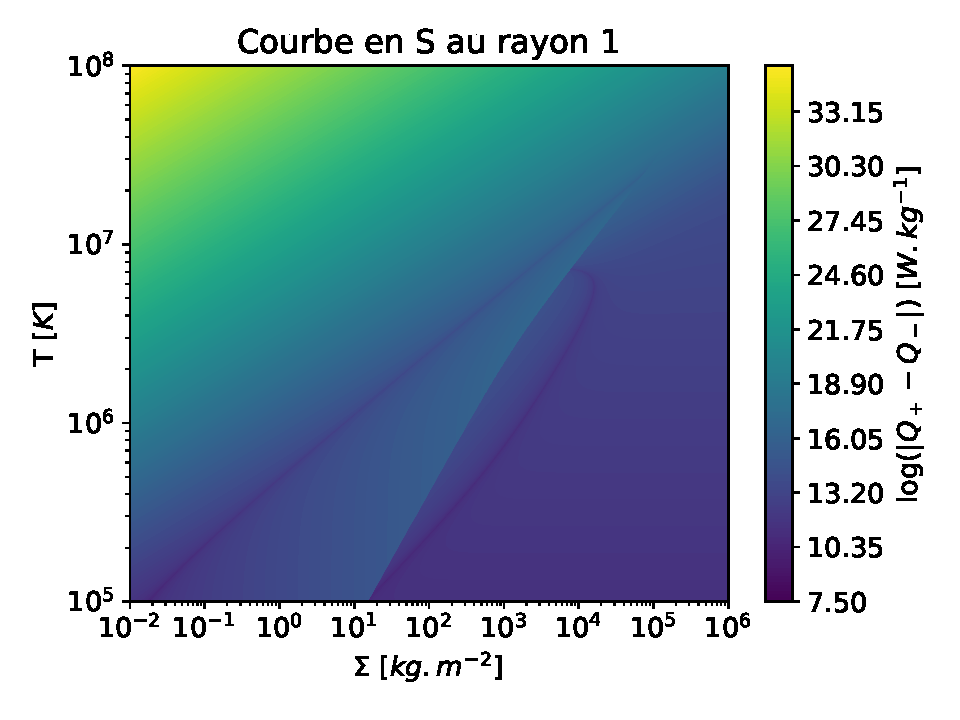
\includegraphics[width=0.49\linewidth]{SLog-1}}
  \hspace{5pt}
  \subfloat[Mesh représentant la différence entre les termes de chauffage et de refroidissement en fonction de la température et de la densité obtenu ainsi que des transitions négative/positive obtenue pour un rayon de $14.4 R_s$ et une masse du trou noir de $10 M_{\odot}$. La zone interne au délimitation des transitions correspond aux valeurs négatives, la zone externe aux valeurs positives]{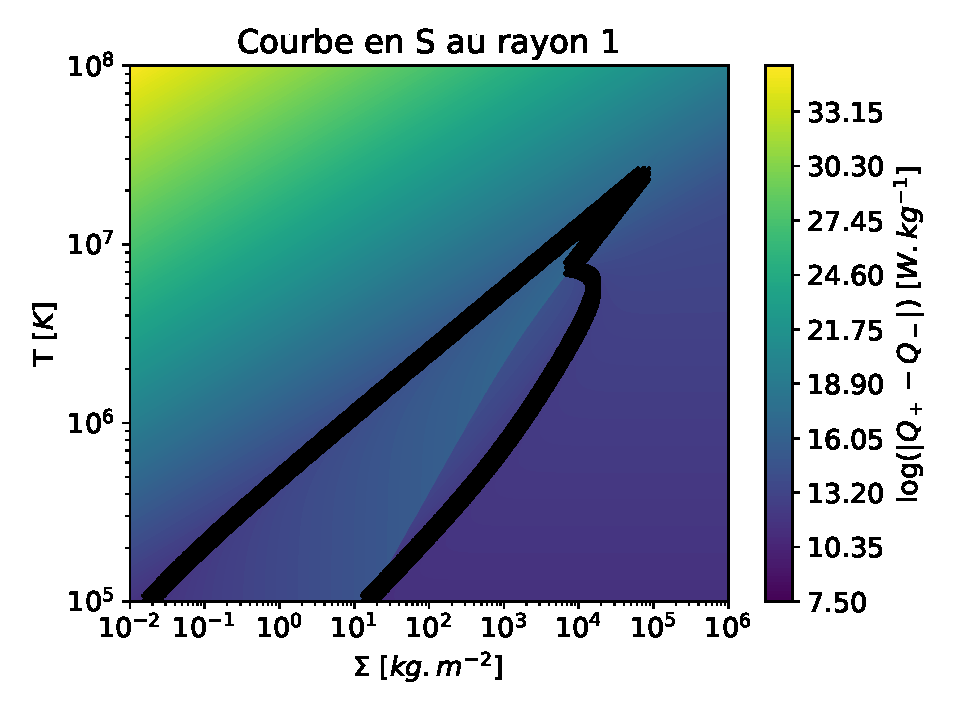
\includegraphics[width=0.49\linewidth]{SLogFrame-1}}
  \caption{Exemples de mesh obtenus pour un même rayon}
\end{figure}
    
\begin{figure}
  \centering
  \subfloat[Mesh représentant la différence entre les termes de chauffage et de refroidissement en fonction de la température et de la densité obtenu pour un rayon de $62.9 R_s$ et une masse du trou noir de $10 M_{\odot}$]{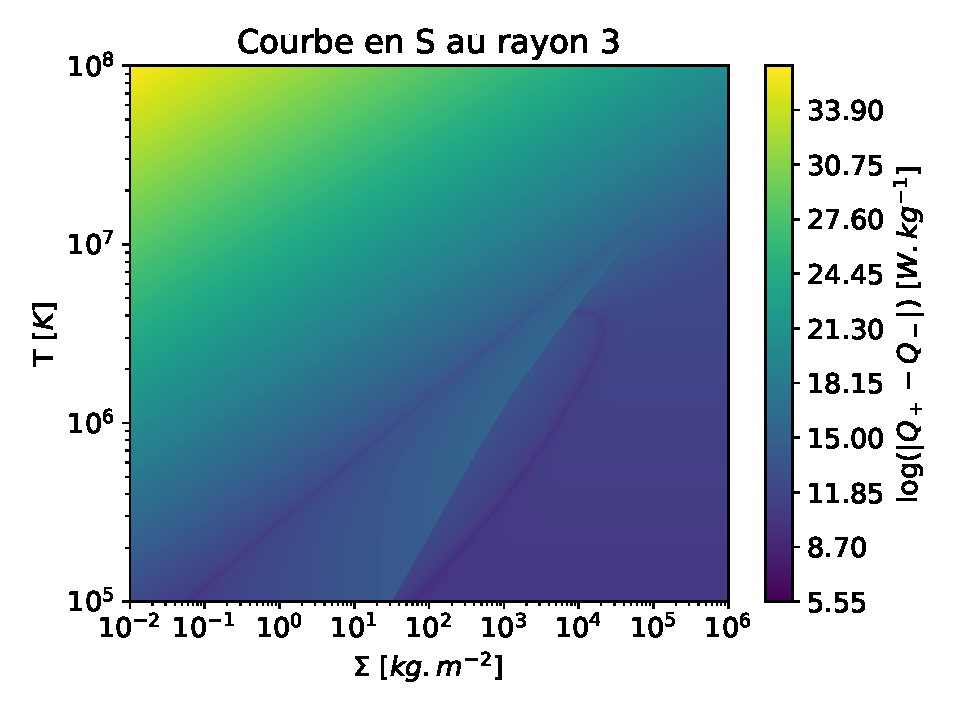
\includegraphics[width=0.49\linewidth]{SLog-3}}
  \hspace{5pt}
  \subfloat[Mesh représentant la différence entre les termes de chauffage et de refroidissement en fonction de la température et de la densité obtenu pour un rayon de $100 R_s$ et une masse du trou noir de $10 M_{\odot}$]{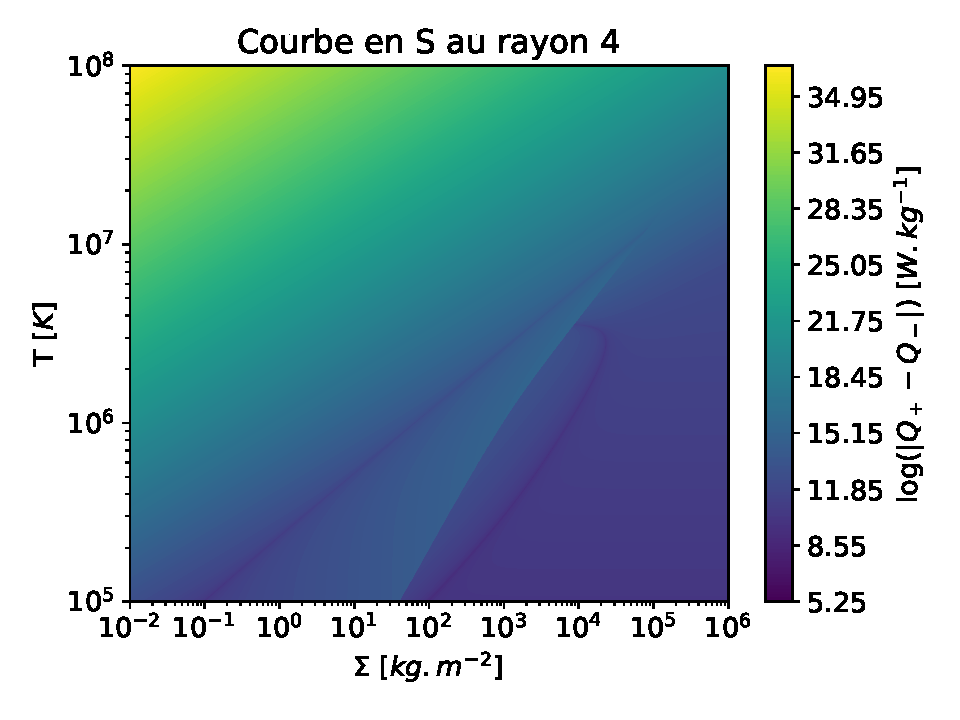
\includegraphics[width=0.49\linewidth]{SLog-4}}
  \caption{Exemples de mesh obtenus pour différents rayon}
\end{figure}

\section{Schémas de discrétisation}

Parmi les équations contenues dans ce modèle, il en existe deux qui impliquent des dérivées temporelles. Ce sont celles régissant d'une part l'évolution de la densité surfacique de masse, et d'autre part la température.
La résolution de ces équations se fait selon les schémas d'Euler, explicite dans un premier temps, puis implicite lorsque nous atteignons une zone instable.

On notera pour toute variable de la forme : $S(x,t) = S(j\text{d}x,n\text{d}t) = S^n_j$ où N est le nombre de pas temporel et J le nombre de pas d'espace tels que $j\in[1,J]$ et $n\in[1,N]$.


\begin{align}
	\frac{\partial S}{\partial t} &= \frac{3}{4 x^2}\frac{\partial^2 \left( \nu S \right)}{\partial t^2} \label{eq:diffSurfacique}\\
	\frac{\partial T}{\partial t} &= \frac{1}{C_v}\left(Q_+ + Q_- + Q_{adv}\right)\label{eq:diffTemperature}\\
	\frac{\partial T}{\partial t} &= \frac{1}{C_v}\left(Q_+ + Q_-\right) + \frac{1}{2}\left[(\Gamma_3 - 1)\frac{T}{S}\left(\frac{3}{2x^2}\frac{\partial^2(\nu S)}{\partial x^2} + v\frac{\partial S/x}{\partial x}\right) - \frac{v}{x}\frac{\partial T}{\partial x}\right]	\label{eq:diffTemperature}
\end{align}

%\begin{align}
%	\frac{\partial u}{\partial t} &= - v \frac{\partial u}{\partial x} \label{eq:diffType1} \\
%	\frac{u^{n+1}_i-u^n_i}{\Delta t} &= -v \frac{u^n_i-u^n_{i-1}}{\Delta x} \\
%	u^{n+1}_i &= u^n_i - \frac{v\Delta t}{\Delta x} \left(u^n_i-u^n_{i-1} \right) \\
%	\lambda &= \frac{v\Delta t}{\Delta x^2} \\
%	u^{n+1}_i &= \lambda u^n_{i-1} + \left(1-\lambda\right) u^n_i \label{eq:explicitDiffType1}
%\end{align}

%\begin{align}
%	\frac{\partial u}{\partial t} &= v \frac{\partial^2 u}{\partial x^2} \label{eq:diffType2} \\
%	\frac{u^{n+1}_i-u^n_i}{\Delta t} &= v \frac{u^n_{i-1}-2u^n_i+u^n_{i+1}}{\Delta x^2} \\
%	u^{n+1}_i &= u^n_i + \frac{v\Delta t}{\Delta x^2} \left(u^n_{i-1}-2u^n_i+u^n_{i+1} \right) \\
%	\lambda &= \frac{v\Delta t}{\Delta x^2} \\
%	u^{n+1}_i &= \lambda u^n_{i-1} + \left(1-2\lambda\right) u^n_i + \lambda u^n_{i+1} \label{eq:explicitDiffType2}
%\end{align}

\subsection{Les conditions aux bords}
Le fait que la masse accrétée par unité de temps est constante doit être traduit dans le code par une condition au bord extérieur. En effet, la variation spatiale de la densité surfacique dépend directement du taux d'accrétion.

\begin{align}
\left.3\pi\frac{\partial}{\partial x}\left(\nu S\right)\right|_{x\text{max}} &= \dot{M_0}\label{S_conditionExt}
\end{align}

En injectant cette équation dans \ref{eq:diffSurfacique}, 

\begin{align}
\left.\frac{\partial S}{\partial t}\right|_{x\text{max}} &= \frac{3}{4x_\text{max}\text{d}x}\left(\frac{\dot{M_0}}{3\pi} - \frac{\partial \nu S}{\partial x}(x_\text{max} - \text{d}x) \right)
\end{align}

C'était ce que nous avions tenté de faire au début mais finalement, il existe une solution plus simple pour exprimer S au bord extérieur, il suffit de développer la dérivée de l'équation \ref{S_conditionExt} :

\begin{align}
S^{n+1}_J &= \frac{1}{\nu_{J-1}^{n+1}} \left( \frac{\dot{M_0}}{3\pi}\Delta x + \nu^{n+1}_{J-1}S_{J-1}^{n+1}\right)\\
 &\approx  \frac{1}{\nu_{J-1}^{n}} \left( \frac{\dot{M_0}}{3\pi}\Delta x + \nu^{n}_{J-1}S_{J-1}^{n+1}\right)\label{condExterne}
\end{align}

On effectue l'approximation que $\nu$ au temps $t$ sera très proche de sa valeur au temps $t+\Delta t$ car cette dernière n'est pas encore calculée.

Ensuite, pour le bord interne qui est la dernière orbite stable du disque d'accrétion, la matière tombe dans le trou noir dès qu'elle franchit cette limite. La condition au bord interne (en $x_\text{min}$) sera donc de fixer la densité surfacique à 0. On peut donc injecter $S_1^n = 0$ dans (\ref{eq:diffSurfacique}) à condition que $\nu$ ne tende pas vers l'infini ne $x_\text{min}$ : 

\begin{align}
S^{n+1}_1 &= S^n_1 + \frac{3\Delta t}{4x_1^2\Delta x^2}\left(\nu_2^nS_2^n - 2\nu_1^nS_1^n +0\right)
\end{align}

En connaissant les valeurs de $\nu$ et $S$ au temps $n$, on en déduit donc les valeurs aux bords au temps $n+1$. Pour toutes les autres valeurs, on suivra les méthodes explicite puis implicite d'Euler.

Par ailleurs, l'équation d'évolution de la température \ref{eq:diffTemperature} s'exprime en fonction des termes de chauffage, et n'a pas besoin de conditions aux bords directement.
Cependant, le terme d'advection $Q_\text{adv}$, s'exprime avec des dérivées spatiales et a donc besoin des conditions aux bords. On utilise exactement les mêmes conditions que pour l'équation sur la densité surfacique.

\subsection{Schéma explicite}
\subsubsection{Écriture du schéma explicite}

Le schéma explicite consiste à exprimer la dérivée spatiale au temps qui précède l'itération en cours. On peut donc directement écrire la densité au temps $t+\Delta t$ en fonction des valeurs que l'on connaît par l'itération précédente.

\begin{align}
 	\frac{S^{n+1}_j - S^n_j}{\Delta t} &= \frac{3}{4x_j^2\Delta x^2}\left(\nu^n_{j+1}S^n_{j+1} - 2\nu_j^nS_j^n + \nu^n_{j-1}S^n_{j-1}\right)\\
	S^{n+1}_j &= S_j^n + \frac{3}{4x_j^2}\frac{\Delta t}{\Delta x^2}\left((\nu S)^n_{j+1} - 2(\nu S)_j^n + (\nu S)^n_{j-1}\right)
\end{align}
On pose $\lambda_j = \frac{3}{4x_j^2}\frac{\Delta t}{\Delta x^2}$
Le tableau colonne $S^{n+1}$ où sont stockées les J valeurs de S s'exprime sous la forme :
\begin{align}
S^{n+1} &= AS^n + B
\end{align}

En prenant en compte les conditions aux bords décrites plus haut, les matrices A et B sont (on note ici $\nu_j = \nu^n_j$) :  
\begin{align}
A&= \begin{pmatrix} 1 - 2\nu_1\lambda_1& \lambda_1\nu_2 & \ldots & (0) \\
	\lambda_2\nu_1 & 1 - 2\nu_2\lambda_2 & \lambda_2\nu_3 & \\
	 \ddots& \ddots& \ddots &\\
	  & \lambda_{J-1}\nu_{J-2} & 1 - 2\nu_{J-1}\lambda_{J-1} & \lambda_{J-1}\nu_{J}\\
	  (0) &  &  \frac{\nu_{J-1}}{\nu_J} & 0
\end{pmatrix}\\
 B &= \begin{pmatrix}  0\\
	\vdots\\
	\frac{\dot{M_0}\Delta x}{3\pi\nu_J}
\end{pmatrix}
\end{align}

\subsubsection{Limite de stabilité des schémas explicites}

\paragraph{Équation sur la température}

L'équation pour la température (Eq. \ref{eq:diffTemperature}) étant similaire à une équation d'advection, son schéma explicite à pour condition de stabilité $\lambda < 1$. En développant on obtient comme condition de stabilité sur le pas de temps l'inéquation \ref{eq:stabTemperature}.

\begin{align}
	\lambda &< 1 \\
	\frac{v}{2 x} \frac{\Delta t}{\Delta x} &< 1 \\
	\Delta t &< \frac{2 x}{v} \Delta x \\
	x \geq 3 R_s \quad & \quad R_s = 1 \\
	\Delta t &< \frac{2}{3 max(v)} \Delta x \label{eq:stabTemperature}	
\end{align}

\paragraph{Équation sur la densité surfacique}

L'équation pour la densité surfacique (Eq. \ref{eq:diffSurfacique}) étant similaire à une équation de diffusion, son schéma explicite à pour condition de stabilité $\lambda < \frac{1}{2}$. En développant on obtient comme condition de stabilité sur le pas de temps l'inéquation \ref{eq:stabSurfacique}.

\begin{align}
	\lambda &< \frac{1}{2} \\
	\frac{3}{4 x^2} \frac{\Delta t}{\Delta x^2} &< \frac{1}{2} \\
	\Delta t &< \frac{2}{3} x^2 \Delta x^2 \\
	x \geq 3 R_s \quad & \quad R_s = 1 \\
	\Delta t &< 2 \Delta x^2 \label{eq:stabSurfacique}	
\end{align}

\subsection{Schéma implicite}

Le schéma implicite consiste à exprimer la dérivée spatiale de (\ref{eq:diffSurfacique}) au temps de l'itération en cours, donc à $t+\Delta t$. On a donc :

\begin{align}
 	\frac{S^{n+1}_j - S^n_j}{\Delta t} &= \frac{3}{4x_j^2\Delta x^2}\left((\nu S)^{n+1}_{j+1} - 2(\nu S)_j^{n+1} + (\nu S)^{n+1}_{j-1}\right)\\
	\intertext{On prendra $\nu^{n+1} \approx \nu^n$ car nous ne connaissons pas la valeur que prendra $\nu$ dans la prochaine itération.}
	S^n_j &= S_j^{n+1} - \frac{3\Delta t}{4x_j^2\Delta x^2}\left(\nu^n_{j+1}S^{n+1}_{j+1} - 2\nu^n_j S_j^{n+1} + \nu^n_{j-1} S^{n+1}_{j-1}\right)\\
\end{align}
On pose $\lambda_j = \frac{3}{4x_j^2}\frac{\Delta t}{\Delta x^2}$
Le tableau colonne $S^n$ où sont stockées les J valeurs de S au temps $t=n\Delta t$ est :
\begin{align}
S^n &= AS^{n+1} + B
\end{align}

En prenant en compte les conditions aux bords décrites plus haut, les matrices A et B sont : (on note encore $\nu_j = \nu^n_j$)
\begin{align}
A&= \begin{pmatrix} 1 + 2\nu_1\lambda_1& -\lambda_1\nu_2 & \ldots & (0) \\
	-\lambda_2\nu_1 & 1 + 2\lambda_2\nu_2 &- \lambda_2\nu_3 & \\
	 \ddots& \ddots& \ddots &\\
	  &- \lambda_{J-1}\nu_{J-2} & 1 + 2\nu_{J-1}\lambda_{J-1} &- \lambda_{J-1}\nu_{J}\\
	  (0) &  & 0 & 0
\end{pmatrix}\\
 B &= \begin{pmatrix}  0\\
	\vdots\\
	\frac{\dot{M_0}\Delta x}{3\pi\nu_J} + \frac{\nu_{J-1}}{\nu_J}S^n_{J-1}
\end{pmatrix}
\end{align}

Il n'est cependant pas possible de résoudre ce système d'équations car la dernière ligne est nulle, le rang de cette matrice n'est donc pas J comme on le souhaiterais. Une solution pour obtenir $S^{n+1}$ est de prendre l'équation au bord externe (\ref{condExterne}) :

\begin{align}
	\nu_J^nS^{n+1}_J - \nu_{J-1}^nS_{J-1}^n &= \Delta x \frac{\dot{M_0}}{3\pi}
\end{align}
Le système suivant est alors résolvable :

\begin{align}
 \begin{pmatrix}1 + 2\nu_1\lambda_1& -\lambda_1\nu_2 & \ldots & (0) \\
	-\lambda_2\nu_1 & 1 + 2\lambda_2\nu_2 &- \lambda_2\nu_3 & \\
	 \ddots& \ddots& \ddots &\\
	  &- \lambda_{J-1}\nu_{J-2} & 1 + 2\nu_{J-1}\lambda_{J-1} &- \lambda_{J-1}\nu_{J}\\
	  (0) &  & -\nu^n_{J-1} & \nu^n_J
 \end{pmatrix}
 \begin{pmatrix}
 S_1^{n+1}\\
 S_2^{n+1}\\
 \vdots\\
 S_J^{n+1}
 \end{pmatrix}
 &=
 \begin{pmatrix}
 S_1^n\\
 \vdots\\
 S_{J-1}^n\\
 \frac{\dot{M_0}\Delta x}{3\pi}
 \end{pmatrix}
 \end{align}

On résoud le système d'équations à l'aide de la libraire Lapack pour obtenir la densité au pas de temps $n+1$. L'avantage du schéma implicite, même s'il est plus coûteux en temps de calcul, est qu'elle est stable pour tout $\lambda$ positif. C'est cette méthode qu'on utilisera dans les parties instables de la courbe en S.

\subsection{Propagation du disque d'accrétion}

L'intérêt d'avoir tracé des courbes en S est de pouvoir situer la propagation du disque sur un graphique dont les axes sont la température et la densité surfacique. La courbe en S sépare deux zones : si un point donné du disque est en dessous de cette courbe, il aura tendance à chauffer, et s'il est au dessus il aura tendance à refroidir. Dans les deux cas, le point du disque se rapprochera de la courbe. Cependant, il est possible d'atteindre une zone instable (en haut à gauche de la courbe) au delà de laquelle le refroidissement provoque un retour en bas de la courbe en S.

Les différents schémas de discrétisation cités plus haut (explicite et implicite) ont chacun des rôles différents. La méthode explicite est simple à mettre en oeuvre. Elle permet dans un premier temps de lancer la simulation en partant de solutions connues et de vérifier que le code donne des résultats cohérents avec la physique du problème. Le point de départ est de prendre les solutions analytiques du livre \cite{king} pour ensuite les faire propager au cours du temps.

\subsubsection{Système physique à plusieurs échelles temporelles}
 
Le disque d'accrétion est un exemple de système qui nécessite un traitement numérique à plusieurs échelles de temps. Les différents phénomènes physiques qui ont lieu dans ce disque se déroulent à des temps caractéristiques qui leurs sont propres. Premièrement, les particules de matières qui sont en rotation autour du trou noir communiquent leur vitesse à leurs voisines, information qui sera transmise au bout d'un certain temps à tout le reste du disque. Plus le disque est visqueux, plus cette information sera vite propagée et le temps visqueux petit.
Deuxièmement, le disque possède un temps dynamique de l'ordre de la durée de rotation sur lui même. Ce temps est comparable au temps thermique, tous deux sont très petits devant le temps visqueux.


\subsubsection{Les pas de temps}
Si le pas de discrétisation de l'espace est choisi comme étant fixe pour toute la durée de la simulation, le pas de temps est choisi parmi les temps caractéristiques du problème.
\paragraph{Le temps thermique} est le temps caractéristique de l'équation de la chaleur (\ref{eq:diffTemperature}). Il vaut :
\begin{align}
t_\text{th} &= \left(\frac{H}{r}\right)^2t_\text{visc} = \left(\frac{H}{x^2}\right)^2t_\text{visc}
\end{align}
Où $t_\text{visc}$ est le temps visqueux. Étant donné que l'épaisseur du disque $H$ est très petite devant n'importe quel rayon, on a toujours $t_\text{th} \ll t_\text{visq}$.
Le temps thermique (sa valeur minimum) sera pris comme pas de temps de la simulation lorsque l'on cherche à faire évoluer doucement le disque qui ira naturellement vers la courbe en S. Il permet de vérifier que le code converge vers ce que nous prévoyons, c'est à dire que le chauffage s'il est positif diminue pour se stabiliser à zéro lorsque nous approchons de la courbe en S.
 \paragraph{Le temps visqueux} est le temps caractéristique de l'équation d'évolution de la densité. Une façon de l'exprimer et celle que nous utilisons est :
 \begin{align}
 t_\text{visc} &= \frac{r^2}{\nu} = \frac{x^4}{\nu}
 \end{align}
 
 \subsubsection{Intégration temporelle}
Faire uniquement des pas de temps visqueux ($\Delta t = t_\text{visc}$) ne rendraient pas compte des processus physiques qui se passent aux échelles de temps thermique. Et inversement, faire uniquement des pas de temps thermiques ($\Delta t = t_\text{visc}$) pourraient rendre compte des processus à échelle de temps plus longue mais nécessiterait beaucoup trop de temps de calcul.
Les pas thermiques sont très petits (de l'ordre de $10^{-6}$ secondes pour un trou noir de dix masses solaires). En lançant uniquement des pas de temps thermiques, le disque évolue lentement et nécessite plusieurs millions d'itérations avant de voir que le taux d'accrétion soit homogène sur tout le disque. 

 Le pas visqueux est enclenché lorsqu'une condition est vérifiée, cette condition indique à quel point le disque est dans un état proche de la courbe en S.
Concrètement, la condition pour déclencher un pas visqueux porte sur la valeur maximale du chauffage $Q^+-Q^-$, en regardant pour toutes les valeurs de $x$. Plus cette valeur est grande, plus nous sommes éloignés de la courbe en S.

\section{Assemblage du code}

Le code s'organise en plusieurs sous-parties. D'une part, de nombreuses équations algébriques sont résolues à chaque itération temporelle. Toutes ces fonctions (telles que la vitesse d'accrétion, le flux radiatif, les différents flux de chaleur, etc...) se basent sur la température $T$ et la densité surfacique $\Sigma$ qui sont obtenues par les schémas d'Euler. Dans l'ordre chronologique, le code effectue les étapes suivantes, programmées dans un fichier "simulationManager.f90" :
\begin{itemize}
	\item{Initialisation du disque}
	\begin{itemize}
		\item{Récupération de la solution analytique en T et S}
		\item{Appel des équations algébriques}
		\item{Écriture dans un fichier de sortie}
	\end{itemize}
	\item{Itération temporelle}
	\begin{itemize}
		\item{Choix du pas de temps (thermique ou visqueux) et conditions de stabilité}
		\item{Calcul de S et T par la méthode d'Euler avec les grandeurs calculées au pas précédent}
		\item{Appel des équations algébriques}
		\item{Écriture dans un fichier de sortie}
	\end{itemize}
	\item{Itération répétée jusqu'à atteindre un nombre d'itérations ou un temps voulu}
\end{itemize}

\section{Résultats et discussions}

\subsection{Évolution spatiale du taux d'accrétion}

\begin{figure}
  \centering
  \includegraphics[width=0.4\linewidth]{accretionRate-stable.pdf}
  \includegraphics[width=0.4\linewidth]{last-accretionRate.pdf}
  \caption{Le taux d'accrétion se stabilisant en quelques heures après le début de l'accétion. Les paramètres sont : un trou noir de 10 masses solaires avec un taux d'accrétion de $5.10^{13}$kg/s. À droite est tracé le taux en fonction du rayon pour le dernier temps de la simulation, après 7000 secondes.}
  \label{accretion rate stabilisation}
\end{figure}



Le but de ce projet est de simuler le comportement d'un disque d'accrétion, et d'observer les grandeurs telles que le flux radiatif, la demi-hauteur, la densité surfacique, etc... Une première approche était de faire tourner la simulation en schéma explicite afin de déceler les erreurs de code. Cette étape de débug a pris un temps beaucoup plus long que prévu. Cependant, nous avons tout de même pu retrouver quelques premiers résultats attendus. En partant de la solution analytique  de \cite{king} trouvée pour un taux d'accrétion faible, on vérifie bien que le disque met plusieurs heures à atteindre un régime stable (figure \ref{accretion rate stabilisation}).

\begin{figure}
  \centering
  \includegraphics[width=0.6\linewidth]{deltaQ-199.pdf}
  \caption{Puissance thermique massique (en Watts/kg) pour un rayon donné (ici le rayon médian du disque) en fonction du temps en se plaçant initialement sous la courbe en S pour un trou noir de dix masses solaires, et un taux d'accrétion de $5.10^{13}$ kg/s}
\end{figure}

On a aussi pu vérifier que la profondeur optique $\tau_{ff}$ est bien supérieure à 1, c'est à dire que l'on est dans le cas où le disque est optiquement épais. En effet la valeur minimale atteinte par $\tau_{ff}$ au cours de cette simulation est de 7,5.


\subsection{Propagation du disque}

La deuxième étape est de simuler sur des temps plus grands et de comparer la propagation avec les courbes en S. Pour les pas de temps plus grands, la limite de stabilité (\ref{eq:stabSurfacique}) nous oblige à utiliser un schéma implicite ou envisager un Crank-Nicholson, dont les conditions de stabilité sont satisfaites si le pas de temps est simplement positif. La figure \ref{scourbe} montre le parcours du disque dans le repère (densité, température) pendant deux heures d'évolution. La courbe en S est affichée en arrière plan de cette propagation. Cela met en évidence le fait que la courbe en S et la propagation se superposent exactement.

\begin{figure}
  \centering
  \includegraphics[width=0.60\linewidth]{SLog-130.pdf}
  \caption{Évolution en (densité, température) du disque au rayon numéro 130 au cours de la même simulation que la figure \ref{accretion rate stabilisation}.}
  \label{scourbe}
\end{figure}

\subsection{Temps de stabilisation du disque en fonction de la masse du trou noir central}

Des simulations on été effectué pour différentes masses de trou noir avec un taux d'accrétion identique. Les figures \ref{fig:mdiscstab} permettent de constater que le taux d'accrétions s'uniformisent plus rapidement avec un trou noir plus massique. Il apparaît alors que plus le trou noir centrale est massique, plus la stabilisation du disque à lieu rapidement pour un même taux d'accrétion. Cependant dans le cas d'une binaire X il est probable qu'un trou noir plus massique augmente le taux d'accrétion.

\begin{figure}
  \centering
    \subfloat[Évolution du taux d’accrétion dans le disque en fonction du temps et du rayon pour un trou noir de $5 M_{\odot}$ et un taux d'accrétion de $5,0 . 10^{13}\ kg.s^{-1}$]{\includegraphics[width=0.49\linewidth]{accretionRate5M}}
  \hspace{5pt}
  \subfloat[Évolution du taux d’accrétion dans le disque en fonction du temps et du rayon pour un trou noir de $10 M_{\odot}$ et un taux d'accrétion de $5,0 . 10^{13}\ kg.s^{-1}$]{\includegraphics[width=0.49\linewidth]{accretionRate10M}}
  \hspace{5pt}
  \subfloat[Évolution du taux d’accrétion dans le disque en fonction du temps et du rayon pour un trou noir de $15 M_{\odot}$ et un taux d'accrétion de $5,0 . 10^{13}\ kg.s^{-1}$]{\includegraphics[width=0.49\linewidth]{accretionRate15M}}
  \caption{Exemples de mesh obtenus pour différents rayon}
  \label{fig:mdiscstab}
\end{figure}


\subsection{Perspectives}

Dans le but d'étudier le comportement du disque à l'approche du point critique de la courbe en S, il faudrait continuer à travailler sur ce code. Notamment, mieux comprendre physiquement ce qui amène le disque à rejoindre un état stable plutôt que de dévier vers la zone instable du point critique. Il faudrait aussi trouver dans le code l'erreur qui amène à des valeurs négatives de pression aux alentours du dixième pas d'espace lors des pas visqueux. De plus, travailler dans la zone stable de la courbe en S comme nous l'avons fait nous permettait de négliger le terme d'advection du transport de chaleur. Parcourir entièrement la courbe en S nécessite de faire plus attention aux hypothèses qui étaient valables jusqu'à présent. Des vérifications ont été faites sur la conservations de la masse qui est au niveau de la précision machine, mais il serait également intéressant de faire des vérifications sur la conservation du moment cinétique.

Un second aspect important qu'il faudrait développer est une meilleur prise en compte de la transition régime à opacité faible vers opacité élevée et vice-versa. Par ailleurs, plusieurs équations ont été simplifié sous l'hypothèse d'un disque optiquement épais ou mince, ce qui n'est pas vérifié en toutes circonstances. 
Si on souhaitait étudier les instabilité du disque, un résultat intéressant serait de prédire les variations d'intensité lumineuse en provenance des disques d'accrétion en connaissant la masse du trou noir et le taux d'accrétion ou inversement : déduire les paramètres physiques du système en observant les variations d'intensité lumineuse provenant du disque.  



\newpage
\bibliography{biblio}
\bibliographystyle{unsrt}

\newgeometry{left=3cm, bottom=2cm}

\newpage
\appendix

\section{Solutions de la dichotomie par méthode d'incrément pour des fonctions tests}
\label{Annexe:dicho}

    \begin{figure}[hb]
        \centering
        \vspace{-20pt}
        \includegraphics[width=0.6\linewidth]{Circle_dicho.png}
        \caption{Zéros trouvés par la routine \textit{sCurveFromDichotomy} depuis une position $(X_0 , Y_0) = (-10 , -250)$ jusqu'à un $Y_{\rm{max}} = 100$ pour une fonction du type $f(X,Y) = X^2 + Y^2 + \alpha$ avec $\alpha \in \mathbb{R}$}
        \label{CircleDicho}
        
        \includegraphics[width=0.6\linewidth]{DiffSquares_dicho.png}
        \caption{Zéros trouvés par la routine \textit{sCurveFromDichotomy} depuis une position $(X_0 , Y_0) = (-75 , -100)$ jusqu'à un $Y_{\rm{max}} = 100$ pour une fonction du type $f(X,Y) = X^2 - Y^2$. La zone pour $X>0$ est à une valeur fixe pour étudier le comportement de la dichotomie face à des discontinuités. }
        \label{Fig:Diffsquares}
    \end{figure}
    
\newpage
\section{Exemple de mesh et de courbes en S à plusieurs rayons}
\label{Annexe:Exemple}

  \begin{figure}[hb]
    \centering
    \includegraphics[width=0.9\linewidth]{Space_pos_neg}
    \caption{Mesh de $\delta Q$ pour un rayon $x \approx r_{\max}/4$. Les valeurs de $\delta Q$ positives et négatives sont représentées séparément. On observe bien des valeurs négatives de au-dessus de la branche du bas et au-dessus de celle du haut, ainsi qu'une transition nette due au passage $\tau_{\rm{eff}} \ll 1$ vers $\tau_{\rm{eff}} \gg 1$.}
    
    \vspace{20pt}
    
    \subfloat[Évolution de la courbe en S à différents rayons. L'indice fait référence au rayon utilisé dans la simulation.]{\label{Fig:3D_Curves}\includegraphics[width=0.45\linewidth]{3D_SCurves_magnified}}
    \hspace{5pt}
    \subfloat[Vue dans le plan $(S,T)$ des 30 premières courbes en S. La température sur la courbe en S semble décroître lorsqu'on s'éloigne du trou noir.]{\label{Fig:2D_Curves}\includegraphics[width=0.45\linewidth]{2D_SCurvespng.png}}
    \caption{Courbes en S pour les 30 rayons les plus proches du trou noir. La branche du haut détectée n'est pas la branche physique (non convergente) mais la branche non-physique.}
    \label{Fig:Curves}
  \end{figure}
    
    
\newpage
\section{Organisation du code}

\begin{itemize}
\item \textbf{constantProgram} contient la variable contrôlant la précision des variables
\item \textbf{constantPhysic} contient des constantes physiques et mathématiques exprimé en SI
\item \textbf{constantSimulation} contient tout les subroutines et fonction pour faire l’adimensionnement ainsi que les constantes physique adimensionnées
\item \textbf{io} contient toutes les subroutines pour charger les paramètres ou effectuer la sorties des données
\item \textbf{algebricEquation} contient toutes les subroutines de calculs des fonctions algébriques
\item \textbf{diffSolver} contient les subroutines pour résoudre les équations différentielles
\item \textbf{sCurve} contient les subroutines pour la dichotomie et les calculs des mesh
\item \textbf{simulationManager} se charge des appels à l'ensemble des surboutines néscéssaire à chaque pas de temps ainsi que de stocké l'ensembles des valeurs de la simulation. Gère également les appels à la sortie, le bouclage sur les pas de temps et les conditions d'arrêts de la simulation
\end{itemize}

\end{document}
